\documentclass[12pt]{article}
\usepackage{pdfpages}

\usepackage{setspace}
\onehalfspacing
\usepackage[a4paper, margin=1in]{geometry}

\title{Case Study 1 – Career, Honesty and Gender}
\author{Graham Pellegrini (Group A)}
\date{\today}

\begin{document}

\maketitle

\section{Question 1}
\textbf{Is it ethically right for Ben to conceal his idea from his employers?}\\

\textit{Group A - No}  
\textit{Group B - Yes}\\

The debate began with Group A asserting that Ben has the right to adhere to his moral beliefs. They argued that the idea is not fully developed, raising ethical and contractual uncertainties.\\

Group B countered that Ben owes the company transparency. They emphasized that critical decisions should not rest solely on one individual, as this poses risks. Committees exist to ensure responsible decision-making and prevent misuse.\\

Group A maintained that the idea remains undeveloped and does not deprive the company of valuable information. They also noted that Ben’s pacifist stance was known upon his hiring, and expectations should align with his beliefs. From a utilitarian perspective, concealing the idea serves the greater good by preventing harm.\\

Group B responded that Ben has benefited from company resources and, in return, owes a contribution. They argued that military advancements can protect soldiers, deter threats, and have broader scientific applications beyond warfare.\\

Group A countered that the contract only applies to fully developed ideas, making the extent of Ben’s obligations unclear. They stressed that employee rights must also be considered and warned of the dangers of an unchecked arms race.\\

Group B reiterated that decisions of this scale should be handled transparently by a committee. Concealment hinders company growth and potential partnerships, while military innovations often lead to public technological benefits. Moreover, if Ben does not develop the idea, someone else might—potentially without ethical considerations.\\

Group A concluded by cautioning against escalating military capabilities, particularly in the current political climate. Since the company is not in the defense sector, Ben was not hired for this purpose. Forcing him to continue working on the idea would likely reduce his productivity and morale. Finally, if technological advancements are inevitable, Ben’s abstention does not hinder progress but allows him to act in accordance with his ethical beliefs.\\

\pagebreak
\section{Question 2}
\textbf{You are a computer engineer and you are assigned on the Manhattan Project. Do you think it is ethical to work on this project?}\\
\textit {Group A - No}
\textit {Group B - Yes}\\

The second debate began with Group A arguing that they would not have contributed to the atomic bomb project, even if it possible meant ending the war sooner. They believed that the moral burden of the deaths would still rest on them. They also noted that Japan was already weakened, and Germany had been defeated, suggesting that alternative measures could have ended the war.\\

Group B countered that after the bomb’s creation, scientists established the Federation of American Scientists to regulate atomic energy and consider public interests. They also highlighted that the research was heavily funded due to the wartime pressures and led to significant scientific advancements.\\

Group A responded that nuclear energy could have been developed without the atomic bomb. They argued that weapons of mass destruction are inherently unethical and unjustifiable.\\

Group B argued that from a utilitarian perspective, if the bomb ended the war and saved more lives than it took, then developing it was ethical. They also noted that from a rule-utilitarian standpoint, no established rule at the time deemed it unethical.\\

Group A countered that even under utilitarianism, the bomb was unjustifiable. They believed that it caused long-term harm to people and the environment, ultimately outweighing any perceived benefit.\\

Group B pointed out that, at the time, it was an arms race and that if the U.S. had not developed the bomb, Germany might have. They also noted that nuclear energy advancements were driven by wartime pressures and funding.\\

Group A noted that scientists failed to consider long-term ethical responsibilities, a principle now emphasized in issues like climate change. They also highlighted that unlike scientists in some other countries, those in the U.S. were not forced to participate—they had a choice.\\

Group B stated that given the urgency of the war, U.S. efforts focused on national defense and preventing further attacks like Pearl Harbor.\\

Group A emphasized that these were the only atomic bombs ever used in warfare and that extensive testing had already provided insights into their effects, making live deployment unnecessary. They also noted that the U.S. is often seen as the hero of the war, yet it remains the only country to have used nuclear weapons in combat, acting in its own self-interest like other nations.\\

Group B concluded that while the bomb was dropped on a civilian area, the Japanese government had received prior warning to evacuate.\\

\pagebreak
\section{Question 3}
\textbf{Positive discrimination in favour of women is often proposed as a measure to address gender imbalance. What are the advantages and disadvantages of such measures?}\\
\textit {Group A - Yes}
\textit {Group B - No}\\

Group B began by arguing that positive discrimination can undermine an individual’s sense of achievement, as they may be recognized not for their merit but to fulfill a quota. Opportunities should arise from personal merit and interest rather than being imposed by an external agenda.\\

Group A countered that positive discrimination considers not only merit but also an individual’s potential. Since men and women have different emotional intelligence, they bring varied skills that may currently be undervalued.\\

Group B argued that positive discrimination is a short-term solution, a mere “band-aid” that does not address the root problem. They believe it may worsen the situation by fostering a perception of tokenism.\\

Group A responded that positive discrimination is necessary because women face unique challenges in life that men do not. Without it, natural biases—such as those arising from life experiences like maternity leave—would continue to create disparities. So positive discrimination is a way to level the playing field.\\

Group B asserted that positive discrimination can negatively impact hiring by prioritizing diversity over competence, potentially lowering workforce quality.\\

Group A concluded that while positive discrimination may seem like a temporary fix, it can have long-term benefits by inspiring future generations of women through relatable role models.\\

Group B argued that positive discrimination attempts to disrupt natural tendencies in career choices, as certain groups may naturally excel in specific fields—such as women in nursing and men in STEM. They noted that positive discrimination can lead to reverse discrimination and that it tries to use a negative idea (discrimination) to achieve a positive outcome.\\

\pagebreak
\section{Question 4}  
\textbf{You are the CEO of a local computer engineering company that employs 150 people. What measures and policies will you put in place to move towards a gender balance?}  

The strongest points discussed were:
\begin{itemize}
    \item Establish clear career advancement criteria to ensure equal opportunities and eliminate ambiguity in promotions and potential discrimination.
    \item Implement blind recruitment, concealing potentially discriminatory information from hiring managers to ensure a fair selection process.
    \item Include both male and female representatives on hiring panels to promote fairness and minimize bias.
    \item Increase the visibility of women in underrepresented fields to inspire others. For example, feature women in STEM on company websites or host industry events highlighting female professionals.
    \item Collaborate with educational institutions to challenge stigmas and encourage equal participation across all fields.
    \item Support diverse employee needs by offering flexible work hours, maternity leave, and childcare facilities.
\end{itemize}

\footnote{The use of ChatGPT was limited to the extent stated in the report. Ideas generated by AI were further developed on to enhance understanding of the topic.}

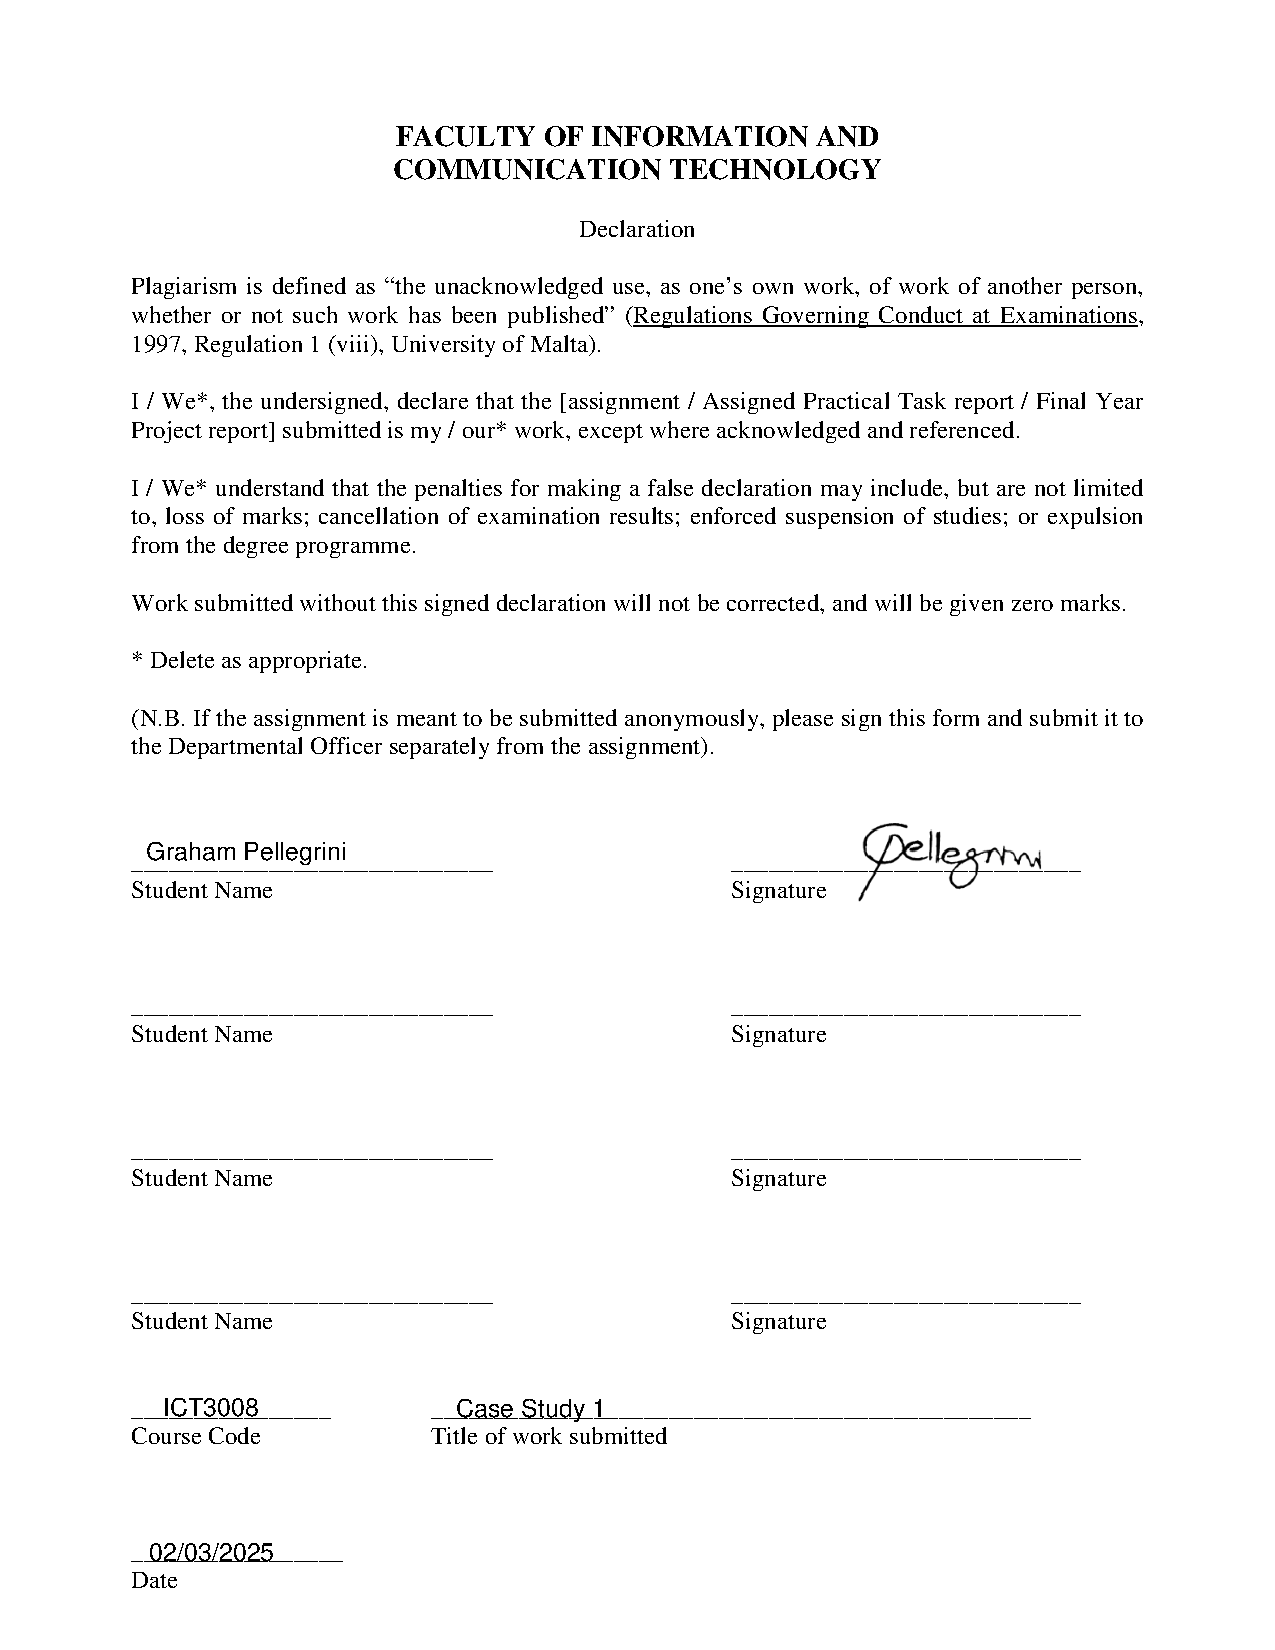
\includepdf[pages=-]{PlagiarismForm_ICT3008_Case1.pdf}


\end{document}